
% Default to the notebook output style

    


% Inherit from the specified cell style.




    
\documentclass[11pt]{article}

    
    
    \usepackage[T1]{fontenc}
    % Nicer default font (+ math font) than Computer Modern for most use cases
    \usepackage{mathpazo}

    % Basic figure setup, for now with no caption control since it's done
    % automatically by Pandoc (which extracts ![](path) syntax from Markdown).
    \usepackage{graphicx}
    % We will generate all images so they have a width \maxwidth. This means
    % that they will get their normal width if they fit onto the page, but
    % are scaled down if they would overflow the margins.
    \makeatletter
    \def\maxwidth{\ifdim\Gin@nat@width>\linewidth\linewidth
    \else\Gin@nat@width\fi}
    \makeatother
    \let\Oldincludegraphics\includegraphics
    % Set max figure width to be 80% of text width, for now hardcoded.
    \renewcommand{\includegraphics}[1]{\Oldincludegraphics[width=.8\maxwidth]{#1}}
    % Ensure that by default, figures have no caption (until we provide a
    % proper Figure object with a Caption API and a way to capture that
    % in the conversion process - todo).
    \usepackage{caption}
    \DeclareCaptionLabelFormat{nolabel}{}
    \captionsetup{labelformat=nolabel}

    \usepackage{adjustbox} % Used to constrain images to a maximum size 
    \usepackage{xcolor} % Allow colors to be defined
    \usepackage{enumerate} % Needed for markdown enumerations to work
    \usepackage{geometry} % Used to adjust the document margins
    \usepackage{amsmath} % Equations
    \usepackage{amssymb} % Equations
    \usepackage{textcomp} % defines textquotesingle
    % Hack from http://tex.stackexchange.com/a/47451/13684:
    \AtBeginDocument{%
        \def\PYZsq{\textquotesingle}% Upright quotes in Pygmentized code
    }
    \usepackage{upquote} % Upright quotes for verbatim code
    \usepackage{eurosym} % defines \euro
    \usepackage[mathletters]{ucs} % Extended unicode (utf-8) support
    \usepackage[utf8x]{inputenc} % Allow utf-8 characters in the tex document
    \usepackage{fancyvrb} % verbatim replacement that allows latex
    \usepackage{grffile} % extends the file name processing of package graphics 
                         % to support a larger range 
    % The hyperref package gives us a pdf with properly built
    % internal navigation ('pdf bookmarks' for the table of contents,
    % internal cross-reference links, web links for URLs, etc.)
    \usepackage{hyperref}
    \usepackage{longtable} % longtable support required by pandoc >1.10
    \usepackage{booktabs}  % table support for pandoc > 1.12.2
    \usepackage[inline]{enumitem} % IRkernel/repr support (it uses the enumerate* environment)
    \usepackage[normalem]{ulem} % ulem is needed to support strikethroughs (\sout)
                                % normalem makes italics be italics, not underlines
    

    
    
    % Colors for the hyperref package
    \definecolor{urlcolor}{rgb}{0,.145,.698}
    \definecolor{linkcolor}{rgb}{.71,0.21,0.01}
    \definecolor{citecolor}{rgb}{.12,.54,.11}

    % ANSI colors
    \definecolor{ansi-black}{HTML}{3E424D}
    \definecolor{ansi-black-intense}{HTML}{282C36}
    \definecolor{ansi-red}{HTML}{E75C58}
    \definecolor{ansi-red-intense}{HTML}{B22B31}
    \definecolor{ansi-green}{HTML}{00A250}
    \definecolor{ansi-green-intense}{HTML}{007427}
    \definecolor{ansi-yellow}{HTML}{DDB62B}
    \definecolor{ansi-yellow-intense}{HTML}{B27D12}
    \definecolor{ansi-blue}{HTML}{208FFB}
    \definecolor{ansi-blue-intense}{HTML}{0065CA}
    \definecolor{ansi-magenta}{HTML}{D160C4}
    \definecolor{ansi-magenta-intense}{HTML}{A03196}
    \definecolor{ansi-cyan}{HTML}{60C6C8}
    \definecolor{ansi-cyan-intense}{HTML}{258F8F}
    \definecolor{ansi-white}{HTML}{C5C1B4}
    \definecolor{ansi-white-intense}{HTML}{A1A6B2}

    % commands and environments needed by pandoc snippets
    % extracted from the output of `pandoc -s`
    \providecommand{\tightlist}{%
      \setlength{\itemsep}{0pt}\setlength{\parskip}{0pt}}
    \DefineVerbatimEnvironment{Highlighting}{Verbatim}{commandchars=\\\{\}}
    % Add ',fontsize=\small' for more characters per line
    \newenvironment{Shaded}{}{}
    \newcommand{\KeywordTok}[1]{\textcolor[rgb]{0.00,0.44,0.13}{\textbf{{#1}}}}
    \newcommand{\DataTypeTok}[1]{\textcolor[rgb]{0.56,0.13,0.00}{{#1}}}
    \newcommand{\DecValTok}[1]{\textcolor[rgb]{0.25,0.63,0.44}{{#1}}}
    \newcommand{\BaseNTok}[1]{\textcolor[rgb]{0.25,0.63,0.44}{{#1}}}
    \newcommand{\FloatTok}[1]{\textcolor[rgb]{0.25,0.63,0.44}{{#1}}}
    \newcommand{\CharTok}[1]{\textcolor[rgb]{0.25,0.44,0.63}{{#1}}}
    \newcommand{\StringTok}[1]{\textcolor[rgb]{0.25,0.44,0.63}{{#1}}}
    \newcommand{\CommentTok}[1]{\textcolor[rgb]{0.38,0.63,0.69}{\textit{{#1}}}}
    \newcommand{\OtherTok}[1]{\textcolor[rgb]{0.00,0.44,0.13}{{#1}}}
    \newcommand{\AlertTok}[1]{\textcolor[rgb]{1.00,0.00,0.00}{\textbf{{#1}}}}
    \newcommand{\FunctionTok}[1]{\textcolor[rgb]{0.02,0.16,0.49}{{#1}}}
    \newcommand{\RegionMarkerTok}[1]{{#1}}
    \newcommand{\ErrorTok}[1]{\textcolor[rgb]{1.00,0.00,0.00}{\textbf{{#1}}}}
    \newcommand{\NormalTok}[1]{{#1}}
    
    % Additional commands for more recent versions of Pandoc
    \newcommand{\ConstantTok}[1]{\textcolor[rgb]{0.53,0.00,0.00}{{#1}}}
    \newcommand{\SpecialCharTok}[1]{\textcolor[rgb]{0.25,0.44,0.63}{{#1}}}
    \newcommand{\VerbatimStringTok}[1]{\textcolor[rgb]{0.25,0.44,0.63}{{#1}}}
    \newcommand{\SpecialStringTok}[1]{\textcolor[rgb]{0.73,0.40,0.53}{{#1}}}
    \newcommand{\ImportTok}[1]{{#1}}
    \newcommand{\DocumentationTok}[1]{\textcolor[rgb]{0.73,0.13,0.13}{\textit{{#1}}}}
    \newcommand{\AnnotationTok}[1]{\textcolor[rgb]{0.38,0.63,0.69}{\textbf{\textit{{#1}}}}}
    \newcommand{\CommentVarTok}[1]{\textcolor[rgb]{0.38,0.63,0.69}{\textbf{\textit{{#1}}}}}
    \newcommand{\VariableTok}[1]{\textcolor[rgb]{0.10,0.09,0.49}{{#1}}}
    \newcommand{\ControlFlowTok}[1]{\textcolor[rgb]{0.00,0.44,0.13}{\textbf{{#1}}}}
    \newcommand{\OperatorTok}[1]{\textcolor[rgb]{0.40,0.40,0.40}{{#1}}}
    \newcommand{\BuiltInTok}[1]{{#1}}
    \newcommand{\ExtensionTok}[1]{{#1}}
    \newcommand{\PreprocessorTok}[1]{\textcolor[rgb]{0.74,0.48,0.00}{{#1}}}
    \newcommand{\AttributeTok}[1]{\textcolor[rgb]{0.49,0.56,0.16}{{#1}}}
    \newcommand{\InformationTok}[1]{\textcolor[rgb]{0.38,0.63,0.69}{\textbf{\textit{{#1}}}}}
    \newcommand{\WarningTok}[1]{\textcolor[rgb]{0.38,0.63,0.69}{\textbf{\textit{{#1}}}}}
    
    
    % Define a nice break command that doesn't care if a line doesn't already
    % exist.
    \def\br{\hspace*{\fill} \\* }
    % Math Jax compatability definitions
    \def\gt{>}
    \def\lt{<}
    % Document parameters
    \title{Ventilation Control}
    
    
    

    % Pygments definitions
    
\makeatletter
\def\PY@reset{\let\PY@it=\relax \let\PY@bf=\relax%
    \let\PY@ul=\relax \let\PY@tc=\relax%
    \let\PY@bc=\relax \let\PY@ff=\relax}
\def\PY@tok#1{\csname PY@tok@#1\endcsname}
\def\PY@toks#1+{\ifx\relax#1\empty\else%
    \PY@tok{#1}\expandafter\PY@toks\fi}
\def\PY@do#1{\PY@bc{\PY@tc{\PY@ul{%
    \PY@it{\PY@bf{\PY@ff{#1}}}}}}}
\def\PY#1#2{\PY@reset\PY@toks#1+\relax+\PY@do{#2}}

\expandafter\def\csname PY@tok@vi\endcsname{\def\PY@tc##1{\textcolor[rgb]{0.10,0.09,0.49}{##1}}}
\expandafter\def\csname PY@tok@nn\endcsname{\let\PY@bf=\textbf\def\PY@tc##1{\textcolor[rgb]{0.00,0.00,1.00}{##1}}}
\expandafter\def\csname PY@tok@m\endcsname{\def\PY@tc##1{\textcolor[rgb]{0.40,0.40,0.40}{##1}}}
\expandafter\def\csname PY@tok@kp\endcsname{\def\PY@tc##1{\textcolor[rgb]{0.00,0.50,0.00}{##1}}}
\expandafter\def\csname PY@tok@mh\endcsname{\def\PY@tc##1{\textcolor[rgb]{0.40,0.40,0.40}{##1}}}
\expandafter\def\csname PY@tok@sh\endcsname{\def\PY@tc##1{\textcolor[rgb]{0.73,0.13,0.13}{##1}}}
\expandafter\def\csname PY@tok@nf\endcsname{\def\PY@tc##1{\textcolor[rgb]{0.00,0.00,1.00}{##1}}}
\expandafter\def\csname PY@tok@mf\endcsname{\def\PY@tc##1{\textcolor[rgb]{0.40,0.40,0.40}{##1}}}
\expandafter\def\csname PY@tok@ch\endcsname{\let\PY@it=\textit\def\PY@tc##1{\textcolor[rgb]{0.25,0.50,0.50}{##1}}}
\expandafter\def\csname PY@tok@fm\endcsname{\def\PY@tc##1{\textcolor[rgb]{0.00,0.00,1.00}{##1}}}
\expandafter\def\csname PY@tok@kc\endcsname{\let\PY@bf=\textbf\def\PY@tc##1{\textcolor[rgb]{0.00,0.50,0.00}{##1}}}
\expandafter\def\csname PY@tok@na\endcsname{\def\PY@tc##1{\textcolor[rgb]{0.49,0.56,0.16}{##1}}}
\expandafter\def\csname PY@tok@ow\endcsname{\let\PY@bf=\textbf\def\PY@tc##1{\textcolor[rgb]{0.67,0.13,1.00}{##1}}}
\expandafter\def\csname PY@tok@gr\endcsname{\def\PY@tc##1{\textcolor[rgb]{1.00,0.00,0.00}{##1}}}
\expandafter\def\csname PY@tok@sc\endcsname{\def\PY@tc##1{\textcolor[rgb]{0.73,0.13,0.13}{##1}}}
\expandafter\def\csname PY@tok@s2\endcsname{\def\PY@tc##1{\textcolor[rgb]{0.73,0.13,0.13}{##1}}}
\expandafter\def\csname PY@tok@cs\endcsname{\let\PY@it=\textit\def\PY@tc##1{\textcolor[rgb]{0.25,0.50,0.50}{##1}}}
\expandafter\def\csname PY@tok@nc\endcsname{\let\PY@bf=\textbf\def\PY@tc##1{\textcolor[rgb]{0.00,0.00,1.00}{##1}}}
\expandafter\def\csname PY@tok@mb\endcsname{\def\PY@tc##1{\textcolor[rgb]{0.40,0.40,0.40}{##1}}}
\expandafter\def\csname PY@tok@si\endcsname{\let\PY@bf=\textbf\def\PY@tc##1{\textcolor[rgb]{0.73,0.40,0.53}{##1}}}
\expandafter\def\csname PY@tok@gi\endcsname{\def\PY@tc##1{\textcolor[rgb]{0.00,0.63,0.00}{##1}}}
\expandafter\def\csname PY@tok@gp\endcsname{\let\PY@bf=\textbf\def\PY@tc##1{\textcolor[rgb]{0.00,0.00,0.50}{##1}}}
\expandafter\def\csname PY@tok@mo\endcsname{\def\PY@tc##1{\textcolor[rgb]{0.40,0.40,0.40}{##1}}}
\expandafter\def\csname PY@tok@ni\endcsname{\let\PY@bf=\textbf\def\PY@tc##1{\textcolor[rgb]{0.60,0.60,0.60}{##1}}}
\expandafter\def\csname PY@tok@kt\endcsname{\def\PY@tc##1{\textcolor[rgb]{0.69,0.00,0.25}{##1}}}
\expandafter\def\csname PY@tok@ge\endcsname{\let\PY@it=\textit}
\expandafter\def\csname PY@tok@bp\endcsname{\def\PY@tc##1{\textcolor[rgb]{0.00,0.50,0.00}{##1}}}
\expandafter\def\csname PY@tok@sb\endcsname{\def\PY@tc##1{\textcolor[rgb]{0.73,0.13,0.13}{##1}}}
\expandafter\def\csname PY@tok@gu\endcsname{\let\PY@bf=\textbf\def\PY@tc##1{\textcolor[rgb]{0.50,0.00,0.50}{##1}}}
\expandafter\def\csname PY@tok@sd\endcsname{\let\PY@it=\textit\def\PY@tc##1{\textcolor[rgb]{0.73,0.13,0.13}{##1}}}
\expandafter\def\csname PY@tok@cm\endcsname{\let\PY@it=\textit\def\PY@tc##1{\textcolor[rgb]{0.25,0.50,0.50}{##1}}}
\expandafter\def\csname PY@tok@nd\endcsname{\def\PY@tc##1{\textcolor[rgb]{0.67,0.13,1.00}{##1}}}
\expandafter\def\csname PY@tok@s1\endcsname{\def\PY@tc##1{\textcolor[rgb]{0.73,0.13,0.13}{##1}}}
\expandafter\def\csname PY@tok@kr\endcsname{\let\PY@bf=\textbf\def\PY@tc##1{\textcolor[rgb]{0.00,0.50,0.00}{##1}}}
\expandafter\def\csname PY@tok@o\endcsname{\def\PY@tc##1{\textcolor[rgb]{0.40,0.40,0.40}{##1}}}
\expandafter\def\csname PY@tok@gs\endcsname{\let\PY@bf=\textbf}
\expandafter\def\csname PY@tok@nl\endcsname{\def\PY@tc##1{\textcolor[rgb]{0.63,0.63,0.00}{##1}}}
\expandafter\def\csname PY@tok@gt\endcsname{\def\PY@tc##1{\textcolor[rgb]{0.00,0.27,0.87}{##1}}}
\expandafter\def\csname PY@tok@dl\endcsname{\def\PY@tc##1{\textcolor[rgb]{0.73,0.13,0.13}{##1}}}
\expandafter\def\csname PY@tok@sr\endcsname{\def\PY@tc##1{\textcolor[rgb]{0.73,0.40,0.53}{##1}}}
\expandafter\def\csname PY@tok@mi\endcsname{\def\PY@tc##1{\textcolor[rgb]{0.40,0.40,0.40}{##1}}}
\expandafter\def\csname PY@tok@s\endcsname{\def\PY@tc##1{\textcolor[rgb]{0.73,0.13,0.13}{##1}}}
\expandafter\def\csname PY@tok@c\endcsname{\let\PY@it=\textit\def\PY@tc##1{\textcolor[rgb]{0.25,0.50,0.50}{##1}}}
\expandafter\def\csname PY@tok@ne\endcsname{\let\PY@bf=\textbf\def\PY@tc##1{\textcolor[rgb]{0.82,0.25,0.23}{##1}}}
\expandafter\def\csname PY@tok@w\endcsname{\def\PY@tc##1{\textcolor[rgb]{0.73,0.73,0.73}{##1}}}
\expandafter\def\csname PY@tok@k\endcsname{\let\PY@bf=\textbf\def\PY@tc##1{\textcolor[rgb]{0.00,0.50,0.00}{##1}}}
\expandafter\def\csname PY@tok@nb\endcsname{\def\PY@tc##1{\textcolor[rgb]{0.00,0.50,0.00}{##1}}}
\expandafter\def\csname PY@tok@no\endcsname{\def\PY@tc##1{\textcolor[rgb]{0.53,0.00,0.00}{##1}}}
\expandafter\def\csname PY@tok@nt\endcsname{\let\PY@bf=\textbf\def\PY@tc##1{\textcolor[rgb]{0.00,0.50,0.00}{##1}}}
\expandafter\def\csname PY@tok@gd\endcsname{\def\PY@tc##1{\textcolor[rgb]{0.63,0.00,0.00}{##1}}}
\expandafter\def\csname PY@tok@nv\endcsname{\def\PY@tc##1{\textcolor[rgb]{0.10,0.09,0.49}{##1}}}
\expandafter\def\csname PY@tok@vg\endcsname{\def\PY@tc##1{\textcolor[rgb]{0.10,0.09,0.49}{##1}}}
\expandafter\def\csname PY@tok@sx\endcsname{\def\PY@tc##1{\textcolor[rgb]{0.00,0.50,0.00}{##1}}}
\expandafter\def\csname PY@tok@kd\endcsname{\let\PY@bf=\textbf\def\PY@tc##1{\textcolor[rgb]{0.00,0.50,0.00}{##1}}}
\expandafter\def\csname PY@tok@c1\endcsname{\let\PY@it=\textit\def\PY@tc##1{\textcolor[rgb]{0.25,0.50,0.50}{##1}}}
\expandafter\def\csname PY@tok@vm\endcsname{\def\PY@tc##1{\textcolor[rgb]{0.10,0.09,0.49}{##1}}}
\expandafter\def\csname PY@tok@se\endcsname{\let\PY@bf=\textbf\def\PY@tc##1{\textcolor[rgb]{0.73,0.40,0.13}{##1}}}
\expandafter\def\csname PY@tok@kn\endcsname{\let\PY@bf=\textbf\def\PY@tc##1{\textcolor[rgb]{0.00,0.50,0.00}{##1}}}
\expandafter\def\csname PY@tok@gh\endcsname{\let\PY@bf=\textbf\def\PY@tc##1{\textcolor[rgb]{0.00,0.00,0.50}{##1}}}
\expandafter\def\csname PY@tok@sa\endcsname{\def\PY@tc##1{\textcolor[rgb]{0.73,0.13,0.13}{##1}}}
\expandafter\def\csname PY@tok@vc\endcsname{\def\PY@tc##1{\textcolor[rgb]{0.10,0.09,0.49}{##1}}}
\expandafter\def\csname PY@tok@cp\endcsname{\def\PY@tc##1{\textcolor[rgb]{0.74,0.48,0.00}{##1}}}
\expandafter\def\csname PY@tok@go\endcsname{\def\PY@tc##1{\textcolor[rgb]{0.53,0.53,0.53}{##1}}}
\expandafter\def\csname PY@tok@err\endcsname{\def\PY@bc##1{\setlength{\fboxsep}{0pt}\fcolorbox[rgb]{1.00,0.00,0.00}{1,1,1}{\strut ##1}}}
\expandafter\def\csname PY@tok@cpf\endcsname{\let\PY@it=\textit\def\PY@tc##1{\textcolor[rgb]{0.25,0.50,0.50}{##1}}}
\expandafter\def\csname PY@tok@il\endcsname{\def\PY@tc##1{\textcolor[rgb]{0.40,0.40,0.40}{##1}}}
\expandafter\def\csname PY@tok@ss\endcsname{\def\PY@tc##1{\textcolor[rgb]{0.10,0.09,0.49}{##1}}}

\def\PYZbs{\char`\\}
\def\PYZus{\char`\_}
\def\PYZob{\char`\{}
\def\PYZcb{\char`\}}
\def\PYZca{\char`\^}
\def\PYZam{\char`\&}
\def\PYZlt{\char`\<}
\def\PYZgt{\char`\>}
\def\PYZsh{\char`\#}
\def\PYZpc{\char`\%}
\def\PYZdl{\char`\$}
\def\PYZhy{\char`\-}
\def\PYZsq{\char`\'}
\def\PYZdq{\char`\"}
\def\PYZti{\char`\~}
% for compatibility with earlier versions
\def\PYZat{@}
\def\PYZlb{[}
\def\PYZrb{]}
\makeatother


    % Exact colors from NB
    \definecolor{incolor}{rgb}{0.0, 0.0, 0.5}
    \definecolor{outcolor}{rgb}{0.545, 0.0, 0.0}



    
    % Prevent overflowing lines due to hard-to-break entities
    \sloppy 
    % Setup hyperref package
    \hypersetup{
      breaklinks=true,  % so long urls are correctly broken across lines
      colorlinks=true,
      urlcolor=urlcolor,
      linkcolor=linkcolor,
      citecolor=citecolor,
      }
    % Slightly bigger margins than the latex defaults
    
    \geometry{verbose,tmargin=1in,bmargin=1in,lmargin=1in,rmargin=1in}
    
    

    \begin{document}
    
    
    \maketitle
    
    

    
    \hypertarget{ux43cux43eux434ux435ux43b-ux43dux430-ux431ux435ux43bux43eux434ux440ux43eux431ux43dux430-ux432ux435ux43dux442ux438ux43bux430ux446ux438ux44f}{%
\subsection{\# Модел на белодробна
вентилация}\label{ux43cux43eux434ux435ux43b-ux43dux430-ux431ux435ux43bux43eux434ux440ux43eux431ux43dux430-ux432ux435ux43dux442ux438ux43bux430ux446ux438ux44f}}

Доклад за курса във ФМИ ``Въведение в изчислителната биология'', доц. П.
Рашков (ИМИ-БАН), 2018-2019г

Беатрис Бонева

    \hypertarget{ux446ux435ux43bux438-ux43dux430-ux43fux440ux43eux435ux43aux442ux430}{%
\subsection{Цели на
проекта}\label{ux446ux435ux43bux438-ux43dux430-ux43fux440ux43eux435ux43aux442ux430}}

\begin{enumerate}
\def\labelenumi{\arabic{enumi}.}
\tightlist
\item
  Моделиране на физиологичния контрол върху количеството въглероден
  двуокис в кръвта
\item
  Изследване на равновесни точки
\end{enumerate}

\begin{itemize}
\tightlist
\item
  Как тялото стабилизира нивото на \(CO_2\)?
\item
  Възможни ли колебания? Кога и от какво възникват?
\end{itemize}

\begin{enumerate}
\def\labelenumi{\arabic{enumi}.}
\setcounter{enumi}{2}
\tightlist
\item
  Можем ли да обясним количествено и качествено някои патологични
  дихателни процеси?
\end{enumerate}

    Известно е, че в кръвта се натрупва въглероден двуокис (\(CO_2\)) като
продукт от нормалния метаболизъм на организма. Иначе казано,
\textbf{въглеродния двуокис се образува от клетките като вторичен
продукт}: 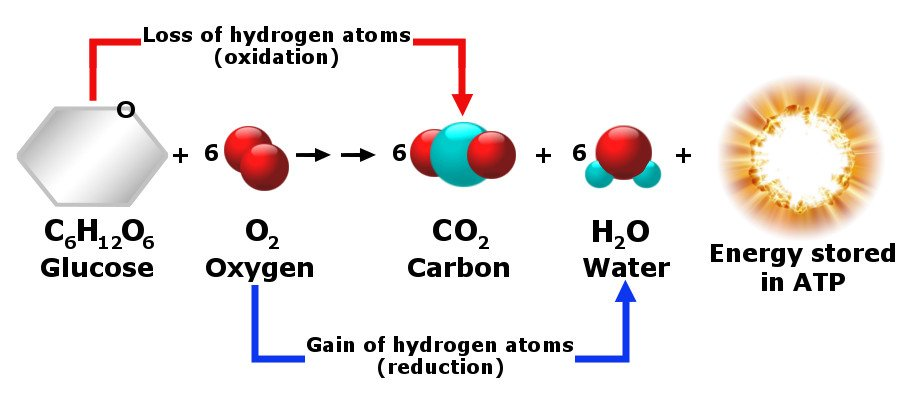
\includegraphics{img/Reactions-of-Cellular-Respiration.jpg}
\emph{\href{https://www.scienceabc.com/humans/why-does-the-human-body-release-carbon-dioxide.html}{Image
Source}}

    За контролиране нивата на \(CO_2\) се грижат \textbf{хеморецепторите} в
мозъчния ствол:
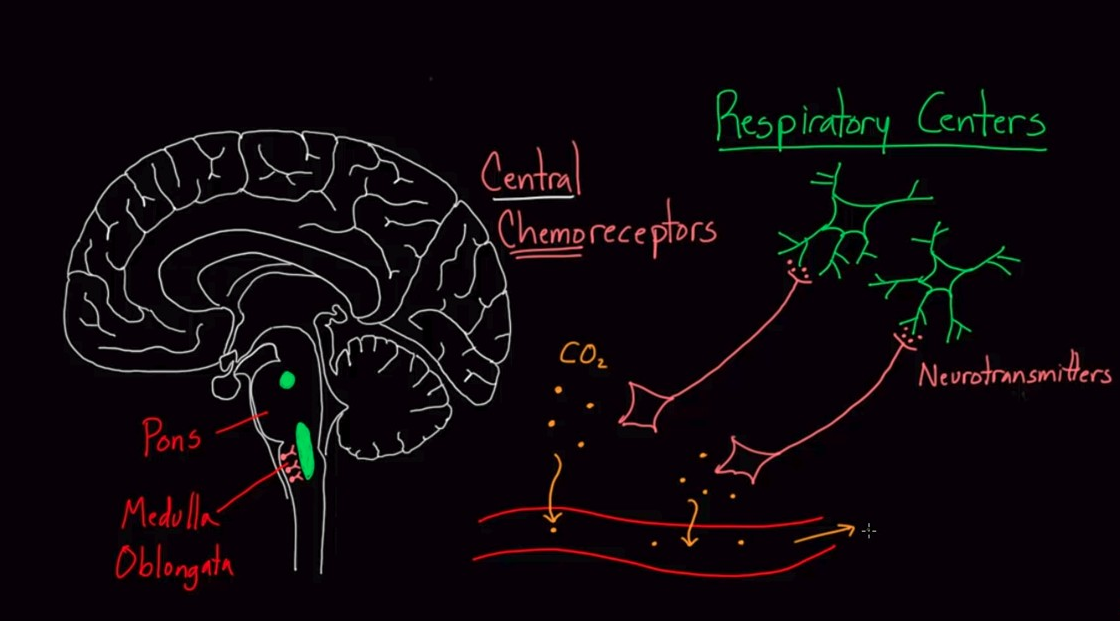
\includegraphics{img/central_chemoreceptors_normal_CO2.jpg}
\emph{\href{https://www.youtube.com/watch?v=lVacrVMmJX8}{Image Source}}

    \textbf{Мостът (pons)} представлява базално издута част на мозъчния
ствол, която се разполага под средния мозък, над гръбначния и пред
малкия мозък. Тази част от мозъчния ствол се нарича още и мост на
Варолий (pons Varolii) - по името на италианския анатом и хирург
Costanzo Varolio (1543-75). Мостът има функционална връзка с малкия
мозък и включва нервни пътища, които предават импулси от крайномозъчната
кора до малкия и гръбначния мозък, и такива, които носят сетивни сигнали
към таламуса.

\textbf{Продълговатият мозък (medulla oblongata)}, е част от мозъчния
ствол на главния мозък и се разполага най-ниско в черепната кухина -
отпред и частично под малкия мозък. Надолу се продължава в гръбначния
мозък, с който имат сходно устройство и функции. За граница между
продълговатия и гръбначния мозък се приема областта, от която излиза
първия гръбначномозъчен нерв, а за граница с надлежащия мост (pons)
отпред служи дълбока напречна бразда - sulcus bulbopontinus, от която
изхождат 6-ти, 7-ми и 8-ми черепномозъчни нерви, а отзад - striae
medullares.

Функцията на продълговатия мозък е свързана с регулация на редица
вегетативни (автономни) процеси като сърдечна дейност, дишане, кръвно
налягане. В него са разположени вегетативни центрове, които
представляват интегрална част на рефлекси като кихане, кашляне,
повръщане и бозаене.

Източник - https://medpedia.framar.bg/

    При високи нива на \(CO_2\) в кръвоносния съд, хеморецепторите не могат
да отделят произведения въглероден двуокис в кръвта и той се натрупва
около тях. Те реагират на повишените нива на \(CO_2\) като изпращат
сигнал по невротрансмитерите към дихателните центрове и по този начин
скоростта на дишане се контролира физиологично.
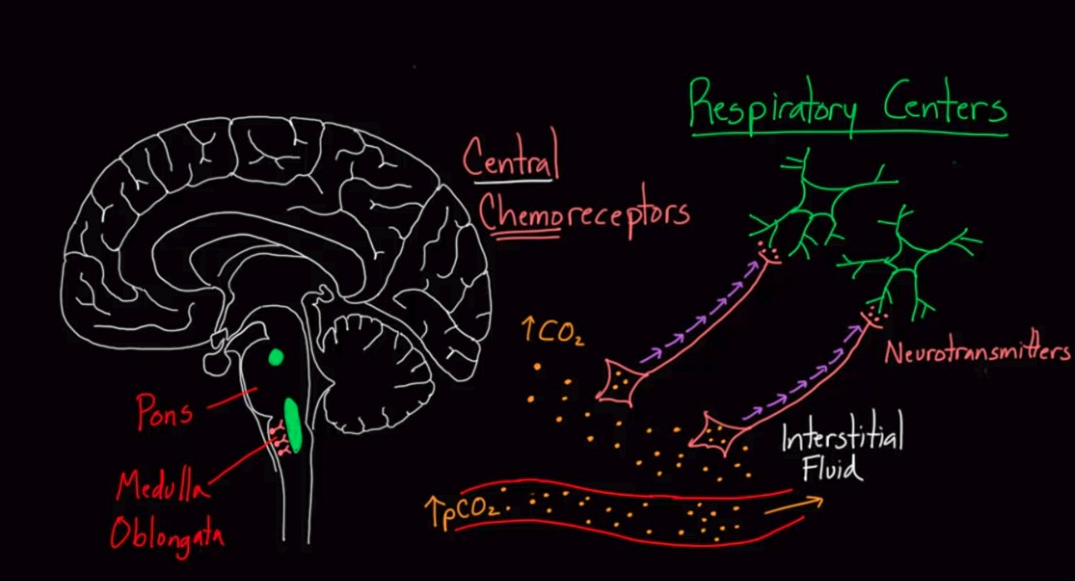
\includegraphics{img/central_chemoreceptors_high_CO2.jpg}

\emph{\href{https://www.youtube.com/watch?v=lVacrVMmJX8}{Image Source}}

    Допускаме, че \(CO_2\) се произвежда от тялото с константна скорост (m)
и се елиминира през белите дробове със скорост пропорционална на
вентилационния обем (\(V_n\)).

Изменението в количеството \(CO_2\) (\(C_n\)) можем да опишем по следния
начин:

\(C_{n+1} - C{n} = m - \beta V_n \quad\)(1)

Вентилационният обем (\(V_n\)), който е контролиран от хеморецепторите,
е монотонно растяща функция спрямо количеството \(CO_2\) в кръвта в
по-ранен момент (\(C_{n-1}\)), т.е. с нарастването на количеството
\(CO_2\), нараства и вентилационния обем. Нека да вземем линейната
функция:

\(V_{n} = \alpha C_{n-1}, \quad \alpha > 0 \quad\) (2)

Всъщност, това ``закъснение'' (зависимостта от по-предходен момент) идва
от времето, необходимо на кръвта да достигне хеморецепторите.

Ако фиксираме \(C\) и \(V\) така, че изменението в количеството \(CO_2\)
(\(C_n\)) и съответно и във вентилационния обем да е 0 (равновесна
точка, \(C_{n+1} = C_n, V_{n+1}=V_n\)), от (1) следва, че:

\(m - \beta \bar{V} = 0 \implies \bar{V} = \frac{m}{\beta}\)

и от (2) намираме равновесната точка и за \(C\):
\(\bar{C} = \frac{m}{\alpha \beta}\).

    Да изследваме равновесната точка за устойчивост:

\$ \textbackslash{}begin\{cases\} C\_\{n+1\} = C\_n - \beta V\_n +
m\textbackslash{} V\_\{n\} = \alpha C\_\{n-1\}
\textbackslash{}end\{cases\}\implies \quad C\_\{n+1\} = C\_n -
\alpha \beta C\_\{n-1\} + m\$

\begin{itemize}
\item
  Ако \(m = 0\), уравнението е хомогенно. Разглеждаме характеристичния
  му полином:

  \(x^2 = x - \alpha \beta\)

  Той има корени \(x_{1;2} = \frac{1 \pm \sqrt{1 - 4 \alpha \beta}}{2}\)

  Тогава общото решение на хомогенното уравнение е: \$A(n) = C\_1
  (\frac{1 + \sqrt{1 - 4 \alpha \beta}}{2})\^{}n + C\_2
  (\frac{1 - \sqrt{1 - 4 \alpha \beta}}{2})\^{}n \$, където \(C_1\) и
  \(C_2\) са константи зависещи от началните условия.
\item
  Ако \(m \neq 0\), уравнение е нехомогенно. Търсим частно решение от
  вида \(B(n) = k, k - const\). Вече знаем, че равновесната точка
  \(\frac{m}{\alpha \beta}\) е решение.

  Следователно, общото решение на нехомогенното уравнение е:
  \(C_n = A(n) + B(n) = C_1 (\frac{1 + \sqrt{1 - 4 \alpha \beta}}{2})^n + C_2 (\frac{1 - \sqrt{1 - 4 \alpha \beta}}{2})^n + \frac{m}{\alpha \beta}\).
\end{itemize}

    Разглеждаме модул от собствените стойности
\(\mid\frac{1 + \sqrt{1 - 4 \alpha \beta}}{2}\mid\) и
\(\mid\frac{1 - \sqrt{1 - 4 \alpha \beta}}{2}\mid\).

\begin{itemize}
\item
  Нека \(4\alpha \beta < 1\).

  От \(\sqrt{1 - 4 \alpha \beta} < 1 \implies\) и двете собствени
  стойности са \(< 1\).

  Следователно, равновесните точки \(\bar{C} = \frac{m}{\alpha \beta}\)
  и \(\bar{V} = \frac{m}{\beta}\) са устойчиви.

  Тоест, нивото на въглероден двуокис и вентилационния обем ще се
  стабилизират в тези точки независимо от началните условия.

  Да видим:
\end{itemize}

    \begin{Verbatim}[commandchars=\\\{\}]
{\color{incolor}In [{\color{incolor}2}]:} \PY{k+kn}{import} \PY{n+nn}{math}
        \PY{k+kn}{import} \PY{n+nn}{numpy} \PY{k}{as} \PY{n+nn}{np}
        \PY{k+kn}{import} \PY{n+nn}{matplotlib}\PY{n+nn}{.}\PY{n+nn}{pyplot} \PY{k}{as} \PY{n+nn}{plt}
\end{Verbatim}


    \begin{Verbatim}[commandchars=\\\{\}]
{\color{incolor}In [{\color{incolor}10}]:} \PY{k}{def} \PY{n+nf}{linear\PYZus{}model}\PY{p}{(}\PY{n}{iterations}\PY{p}{,} \PY{n}{alpha}\PY{o}{=}\PY{k+kc}{None}\PY{p}{,} \PY{n}{beta}\PY{o}{=}\PY{k+kc}{None}\PY{p}{,} \PY{n}{m}\PY{o}{=}\PY{k+kc}{None}\PY{p}{,} \PY{n}{c0}\PY{o}{=}\PY{l+m+mi}{1}\PY{p}{,} \PY{n}{v0}\PY{o}{=}\PY{l+m+mi}{1}\PY{p}{)}\PY{p}{:}
             \PY{n}{result} \PY{o}{=} \PY{p}{[}\PY{p}{[}\PY{n}{c0}\PY{p}{,} \PY{n}{v0}\PY{p}{]}\PY{p}{]}
             \PY{n}{c\PYZus{}current} \PY{o}{=} \PY{n}{c0}
             \PY{n}{v\PYZus{}current} \PY{o}{=} \PY{n}{v0}
             \PY{k}{for} \PY{n}{\PYZus{}} \PY{o+ow}{in} \PY{n+nb}{range}\PY{p}{(}\PY{n}{iterations}\PY{p}{)}\PY{p}{:}
                 \PY{n}{v\PYZus{}next} \PY{o}{=} \PY{n}{alpha} \PY{o}{*} \PY{n}{c\PYZus{}current}
                 \PY{n}{c\PYZus{}next} \PY{o}{=} \PY{n}{c\PYZus{}current} \PY{o}{\PYZhy{}} \PY{n}{beta} \PY{o}{*} \PY{n}{v\PYZus{}current} \PY{o}{+} \PY{n}{m}
                 \PY{n}{result}\PY{o}{.}\PY{n}{append}\PY{p}{(}\PY{p}{[}\PY{n}{c\PYZus{}next}\PY{p}{,} \PY{n}{v\PYZus{}next}\PY{p}{]}\PY{p}{)}
                 \PY{n}{c\PYZus{}current} \PY{o}{=} \PY{n}{c\PYZus{}next}
                 \PY{n}{v\PYZus{}current} \PY{o}{=} \PY{n}{v\PYZus{}next}
             \PY{k}{return} \PY{n}{result}
         
         
         \PY{k}{def} \PY{n+nf}{plot\PYZus{}model}\PY{p}{(}\PY{n}{result}\PY{p}{)}\PY{p}{:}
             \PY{n}{ll} \PY{o}{=} \PY{n}{plt}\PY{o}{.}\PY{n}{plot}\PY{p}{(}\PY{n}{result}\PY{p}{)}
             \PY{n}{xl} \PY{o}{=} \PY{n}{plt}\PY{o}{.}\PY{n}{xlabel}\PY{p}{(}\PY{l+s+s1}{\PYZsq{}}\PY{l+s+s1}{Време}\PY{l+s+s1}{\PYZsq{}}\PY{p}{)}
             \PY{n}{plt}\PY{o}{.}\PY{n}{legend}\PY{p}{(}\PY{n}{ll}\PY{p}{,} \PY{p}{[}\PY{l+s+s2}{\PYZdq{}}\PY{l+s+s2}{Количество \PYZdl{}CO\PYZus{}2\PYZdl{}}\PY{l+s+s2}{\PYZdq{}}\PY{p}{,} \PY{l+s+s2}{\PYZdq{}}\PY{l+s+s2}{Вентилационен обем}\PY{l+s+s2}{\PYZdq{}}\PY{p}{]}\PY{p}{)}
             \PY{n}{plt}\PY{o}{.}\PY{n}{show}\PY{p}{(}\PY{p}{)}
\end{Verbatim}


    \begin{Verbatim}[commandchars=\\\{\}]
{\color{incolor}In [{\color{incolor}12}]:} \PY{n}{plot\PYZus{}model}\PY{p}{(}\PY{n}{linear\PYZus{}model}\PY{p}{(}\PY{l+m+mi}{100}\PY{p}{,} \PY{n}{alpha}\PY{o}{=}\PY{l+m+mf}{0.5}\PY{p}{,} \PY{n}{beta}\PY{o}{=}\PY{l+m+mf}{0.3}\PY{p}{,} \PY{n}{m}\PY{o}{=}\PY{l+m+mf}{1.2}\PY{p}{,} \PY{n}{c0}\PY{o}{=}\PY{l+m+mi}{10}\PY{p}{,} \PY{n}{v0}\PY{o}{=}\PY{l+m+mf}{5.0}\PY{p}{)}\PY{p}{)}
\end{Verbatim}


    \begin{center}
    \adjustimage{max size={0.9\linewidth}{0.9\paperheight}}{output_11_0.png}
    \end{center}
    { \hspace*{\fill} \\}
    
    Виждаме, че количеството въглероден двуокис (\(C_n\)) се стабилизира в
точка \(\frac{m}{\alpha \beta} = \frac{1.2}{0.5*0.3} = 8\), a
вентилационният обем в \$\frac{m}{\beta} = \frac{1.2}{0.3} = 4 \$.

Дори и да променим стойностите на константите \(C_1\) и \(C_2\),
зависещи от началните условия, \(C_n\) и \(V_n\) отново ще се
стабилизират в същите точки:

    \begin{Verbatim}[commandchars=\\\{\}]
{\color{incolor}In [{\color{incolor}14}]:} \PY{n}{plot\PYZus{}model}\PY{p}{(}\PY{n}{linear\PYZus{}model}\PY{p}{(}\PY{l+m+mi}{100}\PY{p}{,} \PY{n}{alpha}\PY{o}{=}\PY{l+m+mf}{0.5}\PY{p}{,} \PY{n}{beta}\PY{o}{=}\PY{l+m+mf}{0.3}\PY{p}{,} \PY{n}{m}\PY{o}{=}\PY{l+m+mf}{1.2}\PY{p}{,} \PY{n}{c0}\PY{o}{=}\PY{l+m+mi}{2}\PY{p}{,} \PY{n}{v0}\PY{o}{=}\PY{l+m+mi}{1}\PY{p}{)}\PY{p}{)}
\end{Verbatim}


    \begin{center}
    \adjustimage{max size={0.9\linewidth}{0.9\paperheight}}{output_13_0.png}
    \end{center}
    { \hspace*{\fill} \\}
    
    \begin{itemize}
\tightlist
\item
  Нека \(4\alpha \beta > 1\). Тогава равновесните точки
  \(\bar{C} = \frac{m}{\alpha \beta}\) и \(\bar{V} = \frac{m}{\beta}\)
  няма да са устойчиви. За някои стойности в този интервал се наблюдават
  колебания в количеството въглероден двуокис и вентилационния обем, а
  за други настъпва хаос.
\end{itemize}

    \begin{Verbatim}[commandchars=\\\{\}]
{\color{incolor}In [{\color{incolor}42}]:} \PY{n}{plot\PYZus{}model}\PY{p}{(}\PY{n}{linear\PYZus{}model}\PY{p}{(}\PY{l+m+mi}{50}\PY{p}{,} \PY{n}{alpha}\PY{o}{=}\PY{l+m+mi}{1}\PY{p}{,} \PY{n}{beta}\PY{o}{=}\PY{l+m+mi}{1}\PY{p}{,} \PY{n}{m}\PY{o}{=}\PY{l+m+mi}{3}\PY{p}{,} \PY{n}{c0}\PY{o}{=}\PY{l+m+mi}{2}\PY{p}{,} \PY{n}{v0}\PY{o}{=}\PY{l+m+mi}{2}\PY{p}{)}\PY{p}{)} \PY{c+c1}{\PYZsh{} alpha*beta = 1}
\end{Verbatim}


    \begin{center}
    \adjustimage{max size={0.9\linewidth}{0.9\paperheight}}{output_15_0.png}
    \end{center}
    { \hspace*{\fill} \\}
    
    \begin{Verbatim}[commandchars=\\\{\}]
{\color{incolor}In [{\color{incolor}47}]:} \PY{n}{plot\PYZus{}model}\PY{p}{(}\PY{n}{linear\PYZus{}model}\PY{p}{(}\PY{l+m+mi}{50}\PY{p}{,} \PY{n}{alpha}\PY{o}{=}\PY{l+m+mf}{1.05}\PY{p}{,} \PY{n}{beta}\PY{o}{=}\PY{l+m+mi}{1}\PY{p}{,} \PY{n}{m}\PY{o}{=}\PY{l+m+mi}{3}\PY{p}{,} \PY{n}{c0}\PY{o}{=}\PY{l+m+mi}{2}\PY{p}{,} \PY{n}{v0}\PY{o}{=}\PY{l+m+mi}{2}\PY{p}{)}\PY{p}{)} \PY{c+c1}{\PYZsh{} alpha*beta = 1.05}
\end{Verbatim}


    \begin{center}
    \adjustimage{max size={0.9\linewidth}{0.9\paperheight}}{output_16_0.png}
    \end{center}
    { \hspace*{\fill} \\}
    
    \begin{Verbatim}[commandchars=\\\{\}]
{\color{incolor}In [{\color{incolor}43}]:} \PY{n}{plot\PYZus{}model}\PY{p}{(}\PY{n}{linear\PYZus{}model}\PY{p}{(}\PY{l+m+mi}{50}\PY{p}{,} \PY{n}{alpha}\PY{o}{=}\PY{l+m+mi}{1}\PY{p}{,} \PY{n}{beta}\PY{o}{=}\PY{l+m+mi}{1}\PY{p}{,} \PY{n}{m}\PY{o}{=}\PY{l+m+mi}{5}\PY{p}{,} \PY{n}{c0}\PY{o}{=}\PY{l+m+mi}{2}\PY{p}{,} \PY{n}{v0}\PY{o}{=}\PY{l+m+mi}{2}\PY{p}{)}\PY{p}{)} \PY{c+c1}{\PYZsh{} alpha*beta = 1}
\end{Verbatim}


    \begin{center}
    \adjustimage{max size={0.9\linewidth}{0.9\paperheight}}{output_17_0.png}
    \end{center}
    { \hspace*{\fill} \\}
    
    Забелязва се, че при нарастване на \(\alpha \beta\) и на \(m\),
колебанията растат.

Можем да заключим, че при нарастване на някое от: - чувствителността на
хеморецепторите; - количеството въглероден двуокис, което тялото
произвежда; системата става нестабилна и може да започне да осцилира.

Тези наблюдения могат да обяснят защо при повишено вътречерепно налягане
(появя се при инсулти, мозъчни тумори, сърдечна недостатъчност и др.)
или хора с надмормено тегло (при които се произвежда повече \(CO_2\)) се
наблюдава неравномерно дишане. Пример за това е патологичното
Чейн-Стоксово дишане. Дълбочината на дихателните движения постепенно се
увеличава, след което също така плавно намалява. Следва период на апнея
и нов цикъл от постепенно задълбочаващи се и след това затихващи
дихателни движения:

\begin{figure}
\centering
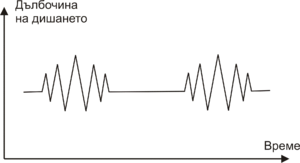
\includegraphics{img/Cheyne_Stokes.png}
\caption{Cheyne\_Stokes.png}
\end{figure}

    Графично, стабилизирането на системата изглежда така:

\begin{figure}
\centering
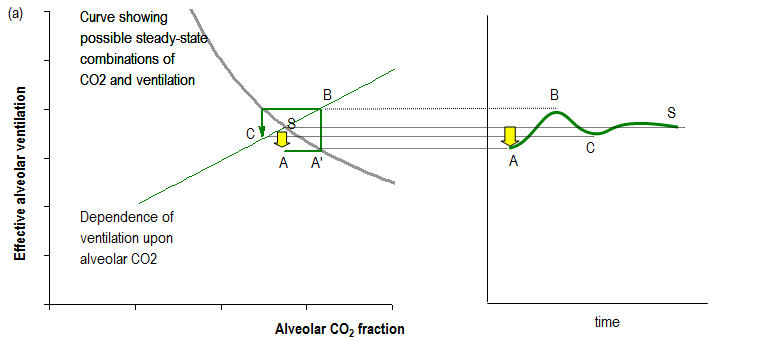
\includegraphics{img/Spiraling-stable.png}
\caption{Spiraling-stable.png}
\end{figure}

Всякакъв малък спад в количеството вентилирано през белите дробове
(\(A\)) води до повишение на количеството \(CO_2\) в кръвта (\(A'\)),
което се засича от хеморецепторите и за да се компенсира, се увеличава
вентилационния обем (B) над равновесната му точка (S) и по този начин
количеството \(CO_2\) се връща в равновесната точка. (Така наречената
``feedback'' система.)

    При патологичното дишане, вентилационният обем се увеличава повече от
необходимото и образува обратно по посока колебание. Ако вторичното
колебание е дори по-голямо от първоначалното, следващото ще е още
по-голямо и т.н., докато не се образуват много големи осцилации и докато
не стигне критична точка като например вентилационният обем да стане 0.
Затова и при Чейн-Стоксово дишане се наблюдава цикличност.

\begin{figure}
\centering
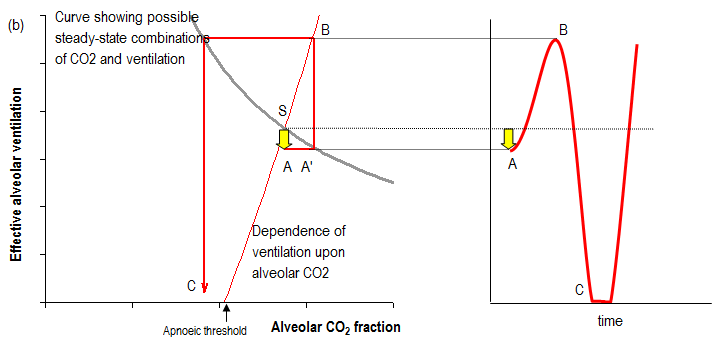
\includegraphics{img/Spiraling-unstable.png}
\caption{Spiraling-unstable.png}
\end{figure}

    Нека количеството \(CO_2\) вентилирано през белите дробове да зависи и
от количеството на \(CO_2\) в сегашния момент, а не само от
венталиционния обем, т.е. \(\mathbf{L(V_n, C_n) = \beta V_n C_n}\).

Тогава

\(\begin{cases}  C_{n+1} = C_n - \beta V_n C_n + m\\  V_{n+1} = \alpha C_{n}  \end{cases}\Leftrightarrow  \begin{cases}  C_{n+1} = C_n - \beta V_n C_n + m\\  V_{n} = \alpha C_{n-1}  \end{cases}\)

Като заместим \(V_n\) в уравнението за \(C_{n+1}\) получаваме едно
уравнение за \(C\):

\(\mathbf{C_{n+1} = C_n - \alpha \beta C_n C_{n-1} + m}\)

    Търсим равновесна точка, т.е. точка за която
\(C_{i+1} = C_i = \bar{C}, \quad \forall i > i' \iff \bar{C} = f(\bar{C})\).
Тогава:

\(f(C) = \bar{C} - \alpha \beta \bar{C}^2 + m\)

\(\bar{C} = f(\bar{C}) \Leftrightarrow \bar{C} = \bar{C} - \alpha \beta \bar{C}^2 + m \implies \alpha \beta \bar{C}^2 = m \implies \bar{C}^2 = \frac{m}{\alpha \beta} \implies \bar{C} = \sqrt{\frac{m}{\alpha \beta}}\)

Изследваме равновесната точка за устойчивост. (За да е устойчива
равновесната точка, трябва \(\mid f'( \bar{C})\mid < 1\).)

\(\mid f'( \bar{C})\mid = \mid \bar{C} - \alpha \beta \bar{C}^2 + m \mid \quad \Leftrightarrow \quad \mid f'( \bar{C})\mid = \mid - 2 \alpha \beta \mid\)

Следователно, равновесната точка

\(\bar{C} = \sqrt{\frac{m}{\alpha \beta}} \text{  е  }  \begin{cases}  \text{устойчива} & \quad \text{за } \alpha \beta < \frac{1}{2}\\  \text{неустойчива} & \quad \text{за } \alpha \beta > \frac{1}{2}  \end{cases}\)

и съответно \(\bar{V} = \alpha \bar{C}\).

Да изследваме модела при тези условия:

    \begin{Verbatim}[commandchars=\\\{\}]
{\color{incolor}In [{\color{incolor}50}]:} \PY{k}{def} \PY{n+nf}{nonlinear\PYZus{}model}\PY{p}{(}\PY{n}{iterations}\PY{p}{,} \PY{n}{alpha}\PY{o}{=}\PY{k+kc}{None}\PY{p}{,} \PY{n}{beta}\PY{o}{=}\PY{k+kc}{None}\PY{p}{,} \PY{n}{m}\PY{o}{=}\PY{k+kc}{None}\PY{p}{,} \PY{n}{c0}\PY{o}{=}\PY{l+m+mi}{1}\PY{p}{,} \PY{n}{v0}\PY{o}{=}\PY{l+m+mi}{1}\PY{p}{)}\PY{p}{:}
             \PY{n}{result} \PY{o}{=} \PY{p}{[}\PY{p}{[}\PY{n}{c0}\PY{p}{,} \PY{n}{v0}\PY{p}{]}\PY{p}{]}
             \PY{n}{c\PYZus{}current} \PY{o}{=} \PY{n}{c0}
             \PY{n}{v\PYZus{}current} \PY{o}{=} \PY{n}{v0}
             \PY{k}{for} \PY{n}{\PYZus{}} \PY{o+ow}{in} \PY{n+nb}{range}\PY{p}{(}\PY{n}{iterations}\PY{p}{)}\PY{p}{:}
                 \PY{n}{c\PYZus{}next} \PY{o}{=} \PY{n}{c\PYZus{}current} \PY{o}{\PYZhy{}} \PY{n}{beta} \PY{o}{*} \PY{n}{c\PYZus{}current} \PY{o}{*} \PY{n}{v\PYZus{}current} \PY{o}{+} \PY{n}{m}
                 \PY{n}{v\PYZus{}next} \PY{o}{=} \PY{n}{alpha} \PY{o}{*} \PY{n}{c\PYZus{}current}
                 \PY{n}{result}\PY{o}{.}\PY{n}{append}\PY{p}{(}\PY{p}{[}\PY{n}{c\PYZus{}next}\PY{p}{,} \PY{n}{v\PYZus{}next}\PY{p}{]}\PY{p}{)}
                 \PY{n}{c\PYZus{}current} \PY{o}{=} \PY{n}{c\PYZus{}next}
                 \PY{n}{v\PYZus{}current} \PY{o}{=} \PY{n}{v\PYZus{}next}
             \PY{k}{return} \PY{n}{result}
\end{Verbatim}


    При \(\alpha \beta < \frac{1}{2}\):

    \begin{Verbatim}[commandchars=\\\{\}]
{\color{incolor}In [{\color{incolor}54}]:} \PY{n}{plot\PYZus{}model}\PY{p}{(}\PY{n}{nonlinear\PYZus{}model}\PY{p}{(}\PY{l+m+mi}{50}\PY{p}{,} \PY{n}{alpha}\PY{o}{=}\PY{l+m+mf}{0.4}\PY{p}{,} \PY{n}{beta}\PY{o}{=}\PY{l+m+mf}{0.4}\PY{p}{,} \PY{n}{m}\PY{o}{=}\PY{l+m+mi}{2}\PY{p}{,} \PY{n}{c0}\PY{o}{=}\PY{l+m+mi}{1}\PY{p}{,} \PY{n}{v0}\PY{o}{=}\PY{l+m+mi}{1}\PY{p}{)}\PY{p}{)}
\end{Verbatim}


    \begin{center}
    \adjustimage{max size={0.9\linewidth}{0.9\paperheight}}{output_25_0.png}
    \end{center}
    { \hspace*{\fill} \\}
    
    \begin{Verbatim}[commandchars=\\\{\}]
{\color{incolor}In [{\color{incolor}98}]:} \PY{n}{plot\PYZus{}model}\PY{p}{(}\PY{n}{nonlinear\PYZus{}model}\PY{p}{(}\PY{l+m+mi}{50}\PY{p}{,} \PY{n}{alpha}\PY{o}{=}\PY{l+m+mf}{0.4}\PY{p}{,} \PY{n}{beta}\PY{o}{=}\PY{l+m+mf}{0.4}\PY{p}{,} \PY{n}{m}\PY{o}{=}\PY{l+m+mi}{4}\PY{p}{,} \PY{n}{c0}\PY{o}{=}\PY{l+m+mi}{1}\PY{p}{,} \PY{n}{v0}\PY{o}{=}\PY{l+m+mi}{1}\PY{p}{)}\PY{p}{)}
\end{Verbatim}


    \begin{center}
    \adjustimage{max size={0.9\linewidth}{0.9\paperheight}}{output_26_0.png}
    \end{center}
    { \hspace*{\fill} \\}
    
    Виждаме, че при по-голямо количество произведен въглероден диоксид от
тялото, колебанията в началото са по-големи и системата се стабилизира
след повече итерации.

    При \(\alpha \beta > \frac{1}{2}\) отново, както при линейната система,
възникват колебания:

    \begin{Verbatim}[commandchars=\\\{\}]
{\color{incolor}In [{\color{incolor}102}]:} \PY{n}{plot\PYZus{}model}\PY{p}{(}\PY{n}{nonlinear\PYZus{}model}\PY{p}{(}\PY{l+m+mi}{100}\PY{p}{,} \PY{n}{alpha}\PY{o}{=}\PY{l+m+mf}{0.8}\PY{p}{,} \PY{n}{beta}\PY{o}{=}\PY{l+m+mf}{0.8}\PY{p}{,} \PY{n}{m}\PY{o}{=}\PY{l+m+mi}{2}\PY{p}{,} \PY{n}{c0}\PY{o}{=}\PY{l+m+mi}{1}\PY{p}{,} \PY{n}{v0}\PY{o}{=}\PY{l+m+mi}{1}\PY{p}{)}\PY{p}{)}
\end{Verbatim}


    \begin{center}
    \adjustimage{max size={0.9\linewidth}{0.9\paperheight}}{output_29_0.png}
    \end{center}
    { \hspace*{\fill} \\}
    
    \begin{Verbatim}[commandchars=\\\{\}]
{\color{incolor}In [{\color{incolor}85}]:} \PY{n}{plot\PYZus{}model}\PY{p}{(}\PY{n}{nonlinear\PYZus{}model}\PY{p}{(}\PY{l+m+mi}{100}\PY{p}{,} \PY{n}{alpha}\PY{o}{=}\PY{l+m+mf}{0.8}\PY{p}{,} \PY{n}{beta}\PY{o}{=}\PY{l+m+mf}{0.8}\PY{p}{,} \PY{n}{m}\PY{o}{=}\PY{l+m+mf}{1.2}\PY{p}{,} \PY{n}{c0}\PY{o}{=}\PY{l+m+mi}{1}\PY{p}{,} \PY{n}{v0}\PY{o}{=}\PY{l+m+mi}{1}\PY{p}{)}\PY{p}{)}
\end{Verbatim}


    \begin{center}
    \adjustimage{max size={0.9\linewidth}{0.9\paperheight}}{output_30_0.png}
    \end{center}
    { \hspace*{\fill} \\}
    
    Интересно е, че за достатъчно малки стойности на произведения \(CO_2\)
(\(m\)) системата може и да успее да се стабилизира, но при по-големи
дори и след голям брой итерации това не се случва:

    \begin{Verbatim}[commandchars=\\\{\}]
{\color{incolor}In [{\color{incolor}108}]:} \PY{n}{plot\PYZus{}model}\PY{p}{(}\PY{n}{nonlinear\PYZus{}model}\PY{p}{(}\PY{l+m+mi}{1000}\PY{p}{,} \PY{n}{alpha}\PY{o}{=}\PY{l+m+mf}{0.8}\PY{p}{,} \PY{n}{beta}\PY{o}{=}\PY{l+m+mf}{0.8}\PY{p}{,} \PY{n}{m}\PY{o}{=}\PY{l+m+mf}{1.6}\PY{p}{,} \PY{n}{c0}\PY{o}{=}\PY{l+m+mi}{1}\PY{p}{,} \PY{n}{v0}\PY{o}{=}\PY{l+m+mi}{1}\PY{p}{)}\PY{p}{)}
\end{Verbatim}


    \begin{center}
    \adjustimage{max size={0.9\linewidth}{0.9\paperheight}}{output_32_0.png}
    \end{center}
    { \hspace*{\fill} \\}
    
    \begin{Verbatim}[commandchars=\\\{\}]
{\color{incolor}In [{\color{incolor}104}]:} \PY{n}{plot\PYZus{}model}\PY{p}{(}\PY{n}{nonlinear\PYZus{}model}\PY{p}{(}\PY{l+m+mi}{100}\PY{p}{,} \PY{n}{alpha}\PY{o}{=}\PY{l+m+mi}{1}\PY{p}{,} \PY{n}{beta}\PY{o}{=}\PY{l+m+mi}{1}\PY{p}{,} \PY{n}{m}\PY{o}{=}\PY{l+m+mf}{1.3}\PY{p}{,} \PY{n}{c0}\PY{o}{=}\PY{l+m+mi}{1}\PY{p}{,} \PY{n}{v0}\PY{o}{=}\PY{l+m+mi}{1}\PY{p}{)}\PY{p}{)}
\end{Verbatim}


    \begin{center}
    \adjustimage{max size={0.9\linewidth}{0.9\paperheight}}{output_33_0.png}
    \end{center}
    { \hspace*{\fill} \\}
    
    \hypertarget{ux441ux438ux433ux43cux43eux438ux434ux43dux430-ux444ux443ux43dux43aux446ux438ux44f-ux437ux430-sc}{%
\subsection{\texorpdfstring{Сигмоидна функция за
\(S(C)\)}{Сигмоидна функция за S(C)}}\label{ux441ux438ux433ux43cux43eux438ux434ux43dux430-ux444ux443ux43dux43aux446ux438ux44f-ux437ux430-sc}}

Mackey и Glass (1977, 1978) разглеждат сигмоидна функция за
чувствителността на хеморецепторите,

\(S(C) = \frac{C^l}{K^l + C^l}\), с параметри
\(l \in \mathbb{N}, K \in \mathbb{R}\).

Нека \(V_{n+1} = V_{max}S(C_n)\), където \(V_{max}\) е максималният
обем.

За \(L(V_n, C_n)\) запазваме нелинейната зависимост
\(L(V_n, C_n) = \beta V_n C_n\).

Тогава

\$\textbackslash{}begin\{cases\} C\_\{n+1\} = C\_n - \beta V\_n C\_n +
m\textbackslash{} V\_\{n+1\} = V\_\{max\}\frac{C_n^l}{K^l + C_n^l}
\textbackslash{}end\{cases\}\Leftrightarrow
\textbackslash{}begin\{cases\} C\_\{n+1\} = C\_n - \beta V\_n C\_n +
m\textbackslash{} V\_\{n\} = V\_\{max\}\frac{C_{n-1}^l}{K^l + C_{n-1}^l}
\textbackslash{}end\{cases\} \$.

Като заместим \(V_n\) в уравнението за \(C_{n+1}\) получаваме едно
уравнение за \(C\):

\(\mathbf{C_{n+1} = C_n - \beta C_n V_{max}\frac{C_{n-1}^l}{K^l + C_{n-1}^l} + m}\)

    Да разгледаме функцията \(S(C) = \frac{C^l}{K^l + C^l}\).

\(l\) се нарича \emph{параметър на кооперативност}, т.е. при \(l > 1\)
свързването на единична молекула към хеморецептора повишава вероятността
за допълнително свързване.

    \begin{Verbatim}[commandchars=\\\{\}]
{\color{incolor}In [{\color{incolor}143}]:} \PY{k}{def} \PY{n+nf}{s}\PY{p}{(}\PY{n}{C}\PY{p}{,} \PY{n}{K}\PY{o}{=}\PY{l+m+mi}{1}\PY{p}{,} \PY{n}{l}\PY{o}{=}\PY{l+m+mi}{0}\PY{p}{)}\PY{p}{:}
              \PY{k}{return} \PY{n}{C}\PY{o}{*}\PY{o}{*}\PY{n}{l} \PY{o}{/} \PY{p}{(}\PY{n}{K}\PY{o}{*}\PY{o}{*}\PY{n}{l} \PY{o}{+} \PY{n}{C}\PY{o}{*}\PY{o}{*}\PY{n}{l}\PY{p}{)}
\end{Verbatim}


    \begin{Verbatim}[commandchars=\\\{\}]
{\color{incolor}In [{\color{incolor}148}]:} \PY{n}{C} \PY{o}{=} \PY{n}{np}\PY{o}{.}\PY{n}{arange}\PY{p}{(}\PY{o}{\PYZhy{}}\PY{l+m+mi}{30}\PY{p}{,} \PY{l+m+mi}{30}\PY{p}{)}
          \PY{n}{f}\PY{p}{,} \PY{p}{(}\PY{n}{ax1}\PY{p}{,} \PY{n}{ax2}\PY{p}{,} \PY{n}{ax3}\PY{p}{)} \PY{o}{=} \PY{n}{plt}\PY{o}{.}\PY{n}{subplots}\PY{p}{(}\PY{l+m+mi}{3}\PY{p}{,} \PY{l+m+mi}{1}\PY{p}{,} \PY{n}{sharex}\PY{o}{=}\PY{k+kc}{True}\PY{p}{)}
          \PY{n}{ax1}\PY{o}{.}\PY{n}{plot}\PY{p}{(}\PY{n}{C}\PY{p}{,} \PY{n}{s}\PY{p}{(}\PY{n}{C}\PY{p}{,} \PY{n}{K}\PY{o}{=}\PY{l+m+mi}{1}\PY{p}{,} \PY{n}{l}\PY{o}{=}\PY{l+m+mi}{0}\PY{p}{)}\PY{p}{)}\PY{p}{;}\PY{n}{ax2}\PY{o}{.}\PY{n}{plot}\PY{p}{(}\PY{n}{C}\PY{p}{,} \PY{n}{s}\PY{p}{(}\PY{n}{C}\PY{p}{,} \PY{n}{K}\PY{o}{=}\PY{l+m+mi}{1}\PY{p}{,} \PY{n}{l}\PY{o}{=}\PY{l+m+mi}{1}\PY{p}{)}\PY{p}{)}\PY{p}{;}\PY{n}{ax3}\PY{o}{.}\PY{n}{plot}\PY{p}{(}\PY{n}{C}\PY{p}{,} \PY{n}{s}\PY{p}{(}\PY{n}{C}\PY{p}{,} \PY{n}{K}\PY{o}{=}\PY{l+m+mi}{1}\PY{p}{,} \PY{n}{l}\PY{o}{=}\PY{l+m+mi}{2}\PY{p}{)}\PY{p}{)}\PY{p}{;}\PY{n}{plt}\PY{o}{.}\PY{n}{show}\PY{p}{(}\PY{p}{)}
\end{Verbatim}


    \begin{Verbatim}[commandchars=\\\{\}]
/usr/local/lib/python3.5/dist-packages/ipykernel\_launcher.py:2: RuntimeWarning: divide by zero encountered in true\_divide
  

    \end{Verbatim}

    \begin{center}
    \adjustimage{max size={0.9\linewidth}{0.9\paperheight}}{output_37_1.png}
    \end{center}
    { \hspace*{\fill} \\}
    
    Функцията е прекъсната в \(-K\), но ние се интересуваме от стойности
по-големи от 0 за \(C\).

    \begin{Verbatim}[commandchars=\\\{\}]
{\color{incolor}In [{\color{incolor}149}]:} \PY{n}{C} \PY{o}{=} \PY{n}{np}\PY{o}{.}\PY{n}{arange}\PY{p}{(}\PY{l+m+mi}{0}\PY{p}{,} \PY{l+m+mi}{50}\PY{p}{)}
          \PY{n}{f}\PY{p}{,} \PY{p}{(}\PY{n}{ax1}\PY{p}{,} \PY{n}{ax2}\PY{p}{,} \PY{n}{ax3}\PY{p}{)} \PY{o}{=} \PY{n}{plt}\PY{o}{.}\PY{n}{subplots}\PY{p}{(}\PY{l+m+mi}{3}\PY{p}{,} \PY{l+m+mi}{1}\PY{p}{,} \PY{n}{sharex}\PY{o}{=}\PY{k+kc}{True}\PY{p}{)}
          \PY{n}{ax1}\PY{o}{.}\PY{n}{plot}\PY{p}{(}\PY{n}{C}\PY{p}{,} \PY{n}{s}\PY{p}{(}\PY{n}{C}\PY{p}{,} \PY{n}{K}\PY{o}{=}\PY{l+m+mi}{82}\PY{p}{,} \PY{n}{l}\PY{o}{=}\PY{l+m+mi}{1}\PY{p}{)}\PY{p}{)}\PY{p}{;}\PY{n}{ax2}\PY{o}{.}\PY{n}{plot}\PY{p}{(}\PY{n}{C}\PY{p}{,} \PY{n}{s}\PY{p}{(}\PY{n}{C}\PY{p}{,} \PY{n}{K}\PY{o}{=}\PY{l+m+mi}{82}\PY{p}{,} \PY{n}{l}\PY{o}{=}\PY{l+m+mi}{2}\PY{p}{)}\PY{p}{)}\PY{p}{;}\PY{n}{ax3}\PY{o}{.}\PY{n}{plot}\PY{p}{(}\PY{n}{C}\PY{p}{,} \PY{n}{s}\PY{p}{(}\PY{n}{C}\PY{p}{,} \PY{n}{K}\PY{o}{=}\PY{l+m+mi}{82}\PY{p}{,} \PY{n}{l}\PY{o}{=}\PY{l+m+mi}{3}\PY{p}{)}\PY{p}{)}\PY{p}{;}\PY{n}{plt}\PY{o}{.}\PY{n}{show}\PY{p}{(}\PY{p}{)}
\end{Verbatim}


    \begin{center}
    \adjustimage{max size={0.9\linewidth}{0.9\paperheight}}{output_39_0.png}
    \end{center}
    { \hspace*{\fill} \\}
    
    \begin{Verbatim}[commandchars=\\\{\}]
{\color{incolor}In [{\color{incolor}116}]:} \PY{k}{def} \PY{n+nf}{model}\PY{p}{(}\PY{n}{iterations}\PY{p}{,} \PY{n}{K}\PY{o}{=}\PY{k+kc}{None}\PY{p}{,} \PY{n}{l}\PY{o}{=}\PY{k+kc}{None}\PY{p}{,} \PY{n}{beta}\PY{o}{=}\PY{k+kc}{None}\PY{p}{,} \PY{n}{m}\PY{o}{=}\PY{k+kc}{None}\PY{p}{,} \PY{n}{v\PYZus{}max}\PY{o}{=}\PY{k+kc}{None}\PY{p}{,} \PY{n}{c0}\PY{o}{=}\PY{k+kc}{None}\PY{p}{)}\PY{p}{:}
              \PY{n}{c\PYZus{}current} \PY{o}{=} \PY{n}{c0}
              \PY{n}{v\PYZus{}current} \PY{o}{=} \PY{n}{v\PYZus{}max} \PY{o}{*} \PY{n}{s}\PY{p}{(}\PY{n}{c\PYZus{}current}\PY{p}{,} \PY{n}{K}\PY{o}{=}\PY{n}{K}\PY{p}{,} \PY{n}{l}\PY{o}{=}\PY{n}{l}\PY{p}{)}
              \PY{n}{result} \PY{o}{=} \PY{p}{[}\PY{p}{[}\PY{n}{c\PYZus{}current}\PY{p}{,} \PY{n}{v\PYZus{}current}\PY{p}{]}\PY{p}{]}
              \PY{k}{for} \PY{n}{\PYZus{}} \PY{o+ow}{in} \PY{n+nb}{range}\PY{p}{(}\PY{n}{iterations}\PY{p}{)}\PY{p}{:}
                  \PY{n}{v\PYZus{}next} \PY{o}{=} \PY{n}{v\PYZus{}max} \PY{o}{*} \PY{n}{s}\PY{p}{(}\PY{n}{c\PYZus{}current}\PY{p}{,} \PY{n}{K}\PY{o}{=}\PY{n}{K}\PY{p}{,} \PY{n}{l}\PY{o}{=}\PY{n}{l}\PY{p}{)}
                  \PY{n}{c\PYZus{}next} \PY{o}{=} \PY{n}{c\PYZus{}current} \PY{o}{\PYZhy{}} \PY{n}{beta} \PY{o}{*} \PY{n}{c\PYZus{}current} \PY{o}{*} \PY{n}{v\PYZus{}current} \PY{o}{+} \PY{n}{m}
                  \PY{n}{result}\PY{o}{.}\PY{n}{append}\PY{p}{(}\PY{p}{[}\PY{n}{c\PYZus{}next}\PY{p}{,} \PY{n}{v\PYZus{}next}\PY{p}{]}\PY{p}{)}
                  \PY{n}{c\PYZus{}current} \PY{o}{=} \PY{n}{c\PYZus{}next}
                  \PY{n}{v\PYZus{}current} \PY{o}{=} \PY{n}{v\PYZus{}next}
              \PY{k}{return} \PY{n}{result}
\end{Verbatim}


    \begin{Verbatim}[commandchars=\\\{\}]
{\color{incolor}In [{\color{incolor}117}]:} \PY{n}{plot\PYZus{}model}\PY{p}{(}\PY{n}{model}\PY{p}{(}\PY{l+m+mi}{100}\PY{p}{,} \PY{n}{K}\PY{o}{=}\PY{l+m+mi}{1}\PY{p}{,} \PY{n}{l}\PY{o}{=}\PY{l+m+mi}{1}\PY{p}{,} \PY{n}{beta}\PY{o}{=}\PY{l+m+mi}{1}\PY{p}{,} \PY{n}{m}\PY{o}{=}\PY{l+m+mi}{2}\PY{p}{,} \PY{n}{v\PYZus{}max}\PY{o}{=}\PY{l+m+mi}{2}\PY{p}{,} \PY{n}{c0}\PY{o}{=}\PY{l+m+mi}{2}\PY{p}{)}\PY{p}{)}
\end{Verbatim}


    \begin{center}
    \adjustimage{max size={0.9\linewidth}{0.9\paperheight}}{output_41_0.png}
    \end{center}
    { \hspace*{\fill} \\}
    
    \begin{Verbatim}[commandchars=\\\{\}]
{\color{incolor}In [{\color{incolor}131}]:} \PY{n}{plot\PYZus{}model}\PY{p}{(}\PY{n}{model}\PY{p}{(}\PY{l+m+mi}{100}\PY{p}{,} \PY{n}{K}\PY{o}{=}\PY{l+m+mi}{1}\PY{p}{,} \PY{n}{l}\PY{o}{=}\PY{l+m+mi}{2}\PY{p}{,} \PY{n}{beta}\PY{o}{=}\PY{l+m+mi}{1}\PY{p}{,} \PY{n}{m}\PY{o}{=}\PY{l+m+mi}{2}\PY{p}{,} \PY{n}{v\PYZus{}max}\PY{o}{=}\PY{l+m+mi}{2}\PY{p}{,} \PY{n}{c0}\PY{o}{=}\PY{l+m+mi}{2}\PY{p}{)}\PY{p}{)}
\end{Verbatim}


    \begin{center}
    \adjustimage{max size={0.9\linewidth}{0.9\paperheight}}{output_42_0.png}
    \end{center}
    { \hspace*{\fill} \\}
    
    \begin{Verbatim}[commandchars=\\\{\}]
{\color{incolor}In [{\color{incolor}138}]:} \PY{n}{plot\PYZus{}model}\PY{p}{(}\PY{n}{model}\PY{p}{(}\PY{l+m+mi}{1000}\PY{p}{,} \PY{n}{K}\PY{o}{=}\PY{l+m+mi}{1}\PY{p}{,} \PY{n}{l}\PY{o}{=}\PY{l+m+mi}{2}\PY{p}{,} \PY{n}{beta}\PY{o}{=}\PY{l+m+mf}{1.1}\PY{p}{,} \PY{n}{m}\PY{o}{=}\PY{l+m+mi}{2}\PY{p}{,} \PY{n}{v\PYZus{}max}\PY{o}{=}\PY{l+m+mi}{2}\PY{p}{,} \PY{n}{c0}\PY{o}{=}\PY{l+m+mi}{1}\PY{p}{)}\PY{p}{)}
\end{Verbatim}


    \begin{center}
    \adjustimage{max size={0.9\linewidth}{0.9\paperheight}}{output_43_0.png}
    \end{center}
    { \hspace*{\fill} \\}
    
    \begin{Verbatim}[commandchars=\\\{\}]
{\color{incolor}In [{\color{incolor}124}]:} \PY{n}{plot\PYZus{}model}\PY{p}{(}\PY{n}{model}\PY{p}{(}\PY{l+m+mi}{100}\PY{p}{,} \PY{n}{K}\PY{o}{=}\PY{l+m+mi}{1}\PY{p}{,} \PY{n}{l}\PY{o}{=}\PY{l+m+mi}{1}\PY{p}{,} \PY{n}{beta}\PY{o}{=}\PY{l+m+mf}{1.5}\PY{p}{,} \PY{n}{m}\PY{o}{=}\PY{l+m+mi}{3}\PY{p}{,} \PY{n}{v\PYZus{}max}\PY{o}{=}\PY{l+m+mi}{2}\PY{p}{,} \PY{n}{c0}\PY{o}{=}\PY{l+m+mi}{2}\PY{p}{)}\PY{p}{)}
\end{Verbatim}


    \begin{center}
    \adjustimage{max size={0.9\linewidth}{0.9\paperheight}}{output_44_0.png}
    \end{center}
    { \hspace*{\fill} \\}
    
    \hypertarget{ux438ux437ux43fux43eux43bux437ux432ux430ux43dux430-ux43bux438ux442ux435ux440ux430ux442ux443ux440ux430}{%
\subsection{Използвана
литература}\label{ux438ux437ux43fux43eux43bux437ux432ux430ux43dux430-ux43bux438ux442ux435ux440ux430ux442ux443ux440ux430}}

\hypertarget{ux43dux430ux443ux447ux43dux438-ux441ux442ux430ux442ux438ux438}{%
\paragraph{Научни
статии}\label{ux43dux430ux443ux447ux43dux438-ux441ux442ux430ux442ux438ux438}}

\begin{itemize}
\tightlist
\item
  M.C. Mackey, L. Glass (1977). Oscillation and chaos in physiological
  control systems, Science 197: 287-289.
\item
  L. Glass, M.C. Mackey (1978). Pathological conditions resulting from
  instabilities in physiological control systems, Ann. NY Acad. Sci.
  316: 214-235.
\item
  M.C. Mackey, J. Milton (1987). Dynamical diseases, Ann. NY Acad. Sci.
  504: 16-32.
\end{itemize}

\hypertarget{ux434ux440ux443ux433ux438-ux438ux437ux442ux43eux447ux43dux438ux446ux438}{%
\paragraph{Други
източници}\label{ux434ux440ux443ux433ux438-ux438ux437ux442ux43eux447ux43dux438ux446ux438}}

\begin{itemize}
\tightlist
\item
  Лекционни материали към курса във ФМИ ``Въведение в изчислителната
  биология'', доц. П. Рашков (ИМИ-БАН), 2018-2019г
\item
  https://en.wikipedia.org/wiki/Cheyne\%E2\%80\%93Stokes\_respiration
\end{itemize}


    % Add a bibliography block to the postdoc
    
    
    
    \end{document}
